% !TEX encoding = UTF-8
% !TEX TS-program = pdflatex
% !TEX root = ../tesi.tex

%**************************************************************
\chapter{Analisi dei requisiti}
\label{cap:analisi-requisiti}
%**************************************************************

%\intro{Breve introduzione al capitolo}\\

\section{Casi d'uso}

Per lo studio dei casi di utilizzo del prodotto sono stati creati dei diagrammi.
I diagrammi dei casi d'uso (in inglese \emph{Use Case Diagram}) sono diagrammi di tipo \gls{uml} dedicati alla descrizione delle funzioni o servizi offerti da un sistema, così come sono percepiti e utilizzati dagli attori che interagiscono col sistema stesso.
Essendo il progetto finalizzato alla creazione di una applicazione per l'automatizzazione di un processo, le interazioni da parte dell'utente devono essere ridotte allo stretto necessario. Per questo motivo i diagrammi d'uso risultano semplici e in numero ridotto.
\newpage

% !TEX encoding = UTF-8
% !TEX TS-program = pdflatex
% !TEX root = ../tesi.tex

\subsection{UC1 - Autenticazione}
\begin{itemize}
  \item \textbf{Identificativo}: UC1
  \item \textbf{Nome}: autenticazione
  \item \textbf{Descrizione grafica}:
\end{itemize}

\begin{figure}[H]
  \centering
  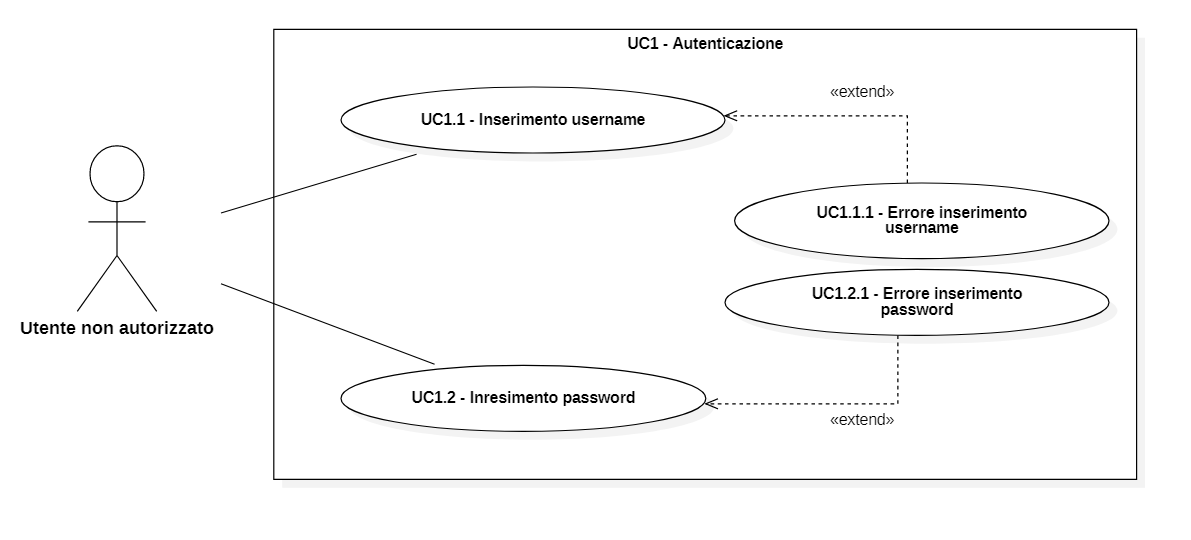
\includegraphics[width=\textwidth]{immagini/usecase/UC1.png}
  \caption{Descrizione grafica caso d'uso UC1}
\end{figure}

\begin{itemize}
  \item \textbf{Attori}
        \begin{itemize}
          \item \textit{Primari}: utente non autorizzato
          \item \textit{Secondari}: Google o Faceebook (???)
        \end{itemize}
  \item \textbf{Precondizione}: l'utente non autenticato si trova sulla pagina di autenticazione.
  \item \textbf{Postcondizione}: l'utente è autenticato.
  \item \textbf{Scenario principale}: l'utente vuole effettuare il login all'applicazione.
  \item \textbf{Scenario secondario}: l'utente non riesce ad autenticarsi a causa di un errore nella procedura. (\textbf{UC1.3})
\end{itemize}

\subsubsection{UC1.1 - Inserimento username}
\begin{itemize}
  \item \textbf{Identificativo}: UC1.1
  \item \textbf{Nome}: inserimento username
  \item \textbf{Descrizione grafica}: (approfondita in UC1)
  \item \textbf{Attori}
        \begin{itemize}
          \item \textit{Primari}: utente non autorizzato
        \end{itemize}
  \item \textbf{Precondizione}: l'utente ha a disposizione una username
  \item \textbf{Postcondizione}: l'utente ha inserito la username.
  \item \textbf{Scenario principale}: l'utente inserisce la username nell'apposito campo di input.
  \item \textbf{Scenario secondario}: l'utente ha inserito una username non corretta che causa un errore. (\textbf{UC1.3})
\end{itemize}

\subsubsection{UC1.1.1 - Errore inserimento username}
\begin{itemize}
  \item \textbf{Identificativo}: UC1.1.1
  \item \textbf{Nome}: errore inserimento username
  \item \textbf{Descrizione grafica}: (approfondita in UC1)
  \item \textbf{Attori}
        \begin{itemize}
          \item \textit{Primari}: utente non autorizzato
        \end{itemize}
  \item \textbf{Precondizione}: la username inserita dall'utente non è correttta.
  \item \textbf{Postcondizione}: l'errore viene mostrato all'utente.
  \item \textbf{Scenario principale}: l'utente inserisce una username non corretta, il sistema segnala l'errore all'utente e mostra nuovamente la maschera di login.
\end{itemize}

\subsubsection{UC1.2 - Inserimento password}
\begin{itemize}
  \item \textbf{Identificativo}: UC1.1
  \item \textbf{Nome}: inserimento password
  \item \textbf{Descrizione grafica}: (approfondita in UC1)
  \item \textbf{Attori}
        \begin{itemize}
          \item \textit{Primari}: utente non autorizzato
        \end{itemize}
  \item \textbf{Precondizione}: l'utente ha a disposizione una password
  \item \textbf{Postcondizione}: l'utente ha inserito la password.
  \item \textbf{Scenario principale}: l'utente inserisce la password nell'apposito campo di input.
  \item \textbf{Scenario secondario}: l'utente ha inserito una password non corretta che causa un errore. (\textbf{UC1.3})
\end{itemize}

\subsubsection{UC1.2.1 - Errore inserimento password}
\begin{itemize}
  \item \textbf{Identificativo}: UC1.2.1
  \item \textbf{Nome}: errore inserimento password
  \item \textbf{Descrizione grafica}: (approfondita in UC1)
  \item \textbf{Attori}
        \begin{itemize}
          \item \textit{Primari}: utente non autorizzato
        \end{itemize}
  \item \textbf{Precondizione}: la password inserita dall'utente non è correttta.
  \item \textbf{Postcondizione}: l'errore viene mostrato all'utente.
  \item \textbf{Scenario principale}: l'utente inserisce una password non corretta, il sistema segnala l'errore all'utente e mostra nuovamente la maschera di login.
\end{itemize}

% \subsubsection{UC1.3 - Errore autenticazione}
% \begin{itemize}
%   \item \textbf{Identificativo}: UC1.3
%   \item \textbf{Nome}: errore autenticazione
%   \item \textbf{Descrizione grafica}: (approfondita in UC1)
%   \item \textbf{Attori}
%         \begin{itemize}
%           \item \textit{Primari}: utente non autorizzato
%         \end{itemize}
%   \item \textbf{Precondizione}: il sitema di autenticazione riceve la richiesta da parte dell'utente.
%   \item \textbf{Postcondizione}: il sistema comunica all'utente l'errore avvenuto, viene riproposta la maschera di login.
%   \item \textbf{Scenario principale}: la richiesta di autenticazione non viene gestita dal sistema che comunica l'errore avvenuto all'utente e mostra nuovamente la maschera di login per un nuovo tentativo.
% \end{itemize}
\newpage
% !TEX encoding = UTF-8
% !TEX TS-program = pdflatex
% !TEX root = ../tesi.tex

\subsection{UC2 - Lettura dati da CD}
\begin{itemize}
  \item \textbf{Identificativo}: UC2
  \item \textbf{Nome}: lettura dati da CD
  \item \textbf{Descrizione grafica}:
\end{itemize}

\begin{figure}[H]
  \centering
  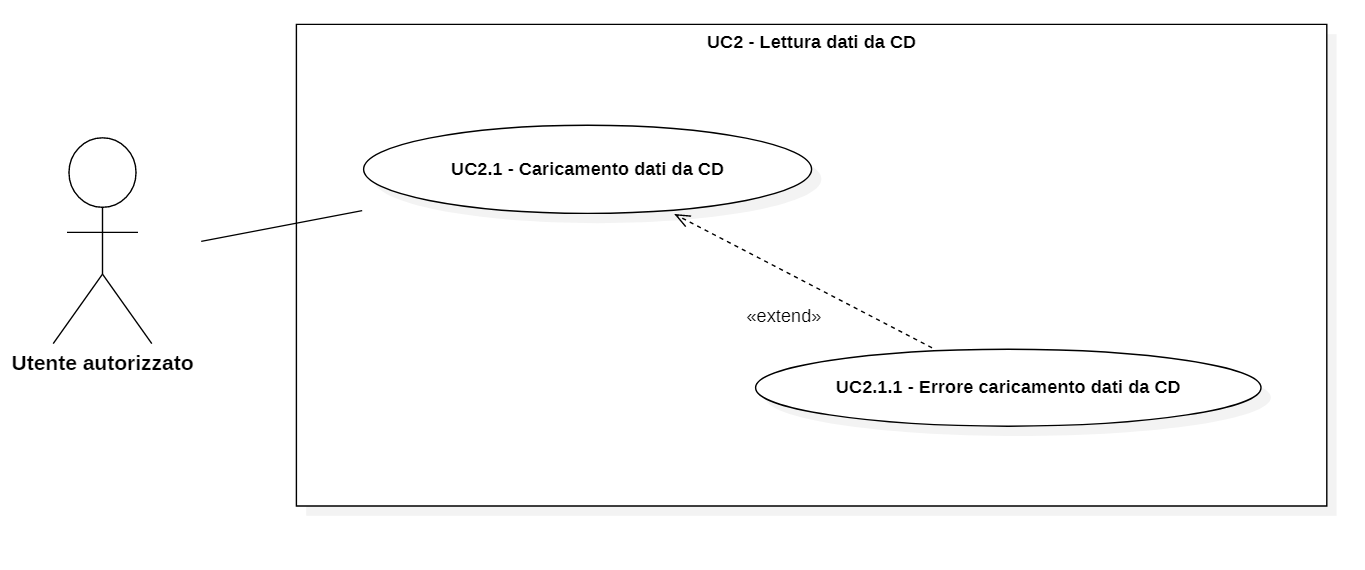
\includegraphics[width=\textwidth]{immagini/usecase/UC2.png}
  \caption{Descrizione grafica caso d'uso UC2}
\end{figure}

\begin{itemize}
  \item \textbf{Attori}
        \begin{itemize}
          \item \textit{Primari}: utente autorizzato
        \end{itemize}
  \item \textbf{Precondizione}: l'utente autorizzato si trova nella pagina per il caricamento dei dati.
  \item \textbf{Postcondizione}: l'utente ha caricato i dati da CD.
  \item \textbf{Scenario principale}: l'utente premendo sull'apposito bottone può caricare i file contenuti nel CD di interesse e li visualizza (\textbf{UC3}).
\end{itemize}

\subsubsection{UC2.1 - Caricamento dati da CD}
\begin{itemize}
  \item \textbf{Identificativo}: UC2.1
  \item \textbf{Nome}: caricamento dati da CD
  \item \textbf{Descrizione grafica}: (approfondita in UC2)
  \item \textbf{Attori}
        \begin{itemize}
          \item \textit{Primari}: utente autorizzato
        \end{itemize}
  \item \textbf{Precondizione}: l'utente ha richiesto il caricamento di una cartella contenente i file del CD.
  \item \textbf{Postcondizione}: i file sono stati caricati nell'applicazione.
  \item \textbf{Scenario principale}: l'utente richiede il caricamento di una cartella contenente i file del CD premendo sull'apposito bottone.
  \item \item \textbf{Scenario secondario}: il sistema riscontra un errore nella procedura di caricamento dei dati. (\textbf{UC2.1})
\end{itemize}

\subsubsection{UC2.1.1 - Errore caricamento dati da CD}
\begin{itemize}
  \item \textbf{Identificativo}: UC2.1
  \item \textbf{Nome}: errore caricamento dati da CD
  \item \textbf{Descrizione grafica}: (approfondita in UC2)
  \item \textbf{Attori}
        \begin{itemize}
          \item \textit{Primari}: utente autorizzato
        \end{itemize}
  \item \textbf{Precondizione}: l'utente ha tentato di caricare i dati.
  \item \textbf{Postcondizione}: l'errore viene mostrato all'utente.
  \item \textbf{Scenario principale}: il sistema non è riuscito a gestire la richiesta di caricamento dei dati da parte dell'utente.
\end{itemize}
\newpage
% !TEX encoding = UTF-8
% !TEX TS-program = pdflatex
% !TEX root = ../tesi.tex

\subsection{UC3 - Visualizzazione file}
\begin{itemize}
  \item \textbf{Identificativo}: UC3
  \item \textbf{Nome}: visualizzazione file
  \item \textbf{Descrizione grafica}:
\end{itemize}

\begin{figure}[h]
  \centering
  %  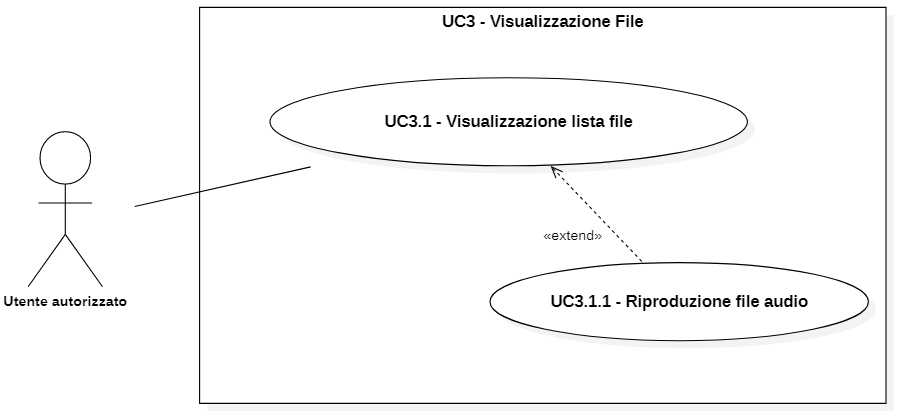
\includegraphics[scale=0.50]{images/UC3.png}
  \caption{Descrizione grafica caso d'uso UC3}
\end{figure}

\begin{itemize}
  \item \textbf{Attori}
        \begin{itemize}
          \item \textit{Primari}: utente autorizzato
        \end{itemize}
  \item \textbf{Precondizione}: l'utente si trova sulla pagina per il caricamento dati, che ha già effettuato correttamente.
  \item \textbf{Postcondizione}: l'utente visualizza i file e i relativi metadati caricati.
  \item \textbf{Scenario principale}: l'utente ha caricato correttamente i dati, questi vengono visualizzati con una lista di file ognuno con i relativi metadati.
  \item \textbf{Scenario secondario}: l'utente può visualizzare ed elaborare i metadati relativi ad ogni file \textbf{UC5}.
\end{itemize}

\subsubsection{UC3.1 - Visualizzazione lista file}
\begin{itemize}
  \item \textbf{Identificativo}: UC3.1
  \item \textbf{Nome}: visualizzazione lista file
  \item \textbf{Descrizione grafica}: (approfondita in UC3)
  \item \textbf{Attori}
        \begin{itemize}
          \item \textit{Primari}: utente autorizzato
        \end{itemize}
  \item \textbf{Precondizione}: l'utente si trova sulla pagina per il caricamento dati, che ha già effettuato correttamente.
  \item \textbf{Postcondizione}: l'utente visualizza la lista dei file ognuno con i relativi metadati.
  \item \textbf{Scenario principale}: l'utente visualizza la lista dei file e può visualizzare la lista dei metadati associati.
  \item \textbf{Scenario secondario}: l'utente può riprodurre i file audio \textbf{UC3.1.1}.
\end{itemize}

\subsubsection{UC3.1.1 - Riproduzione audio file}
\begin{itemize}
  \item \textbf{Identificativo}: UC3.1.1
  \item \textbf{Nome}: riproduzione audio file
  \item \textbf{Descrizione grafica}: (approfondita in UC3)
  \item \textbf{Attori}
        \begin{itemize}
          \item \textit{Primari}: utente autorizzato
        \end{itemize}
  \item \textbf{Precondizione}: l'utente si trova sulla pagina per il caricamento dati, che ha già effettuato correttamente.
  \item \textbf{Postcondizione}: il file audio viene riprodotto.
  \item \textbf{Scenario principale}: l'utente comanda il riproduttore audio con gli appositi comandi play/pause.
\end{itemize}

[Manca visualizzazione/modifica codici procedimenti da capire come gestire questo caso d'uso]
% !TEX encoding = UTF-8
% !TEX TS-program = pdflatex
% !TEX root = ../tesi.tex

\begin{usecase}{4}{Visualizzazione Dati ordinati per Procedimenti}
  \usecaseactors{Utente autorizzato}
  \usecasepre{L'utente si trova all'interno dell'applicazione}
  \usecasedesc{Permette la visualizzazione dei dati caricati da CD}
  \usecasepost{L'utente può visualizzare i dati caricati da CD ordinati per procedimenti}
  \label{uc:visualizzazione-dati-procedimenti}
\end{usecase}


\subsection{UC4 - Visualizzazione dati ordinati per procedimenti}
\begin{itemize}
  \item \textbf{Identificativo}: UC4
  \item \textbf{Nome}: visualizzazione dati ordinati per procedimenti
  \item \textbf{Descrizione grafica}:
\end{itemize}

\begin{figure}[h]
  \centering
  %  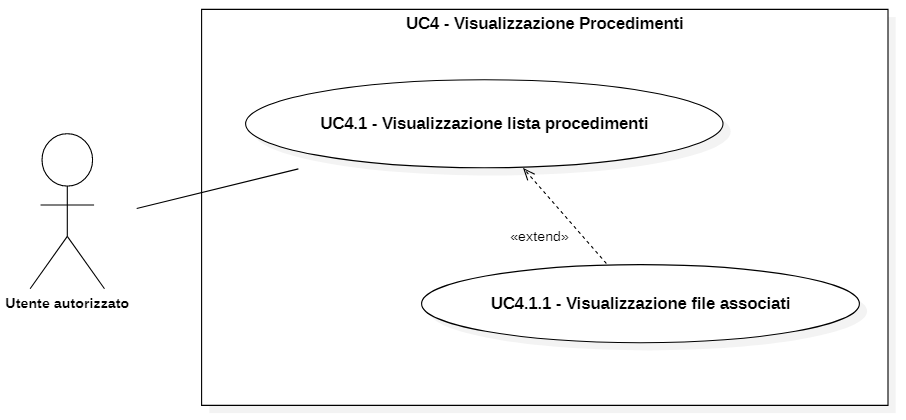
\includegraphics[scale=0.50]{images/UC4.png}
  \caption{Descrizione grafica caso d'uso UC4}
\end{figure}

\begin{itemize}
  \item \textbf{Attori}
        \begin{itemize}
          \item \textit{Primari}: utente autorizzato
        \end{itemize}
  \item \textbf{Precondizione}: l'utente si trova sulla pagina per il caricamento dati, che ha già effettuato correttamente.
  \item \textbf{Postcondizione}: l'utente visualizza i dati caricati sull'applicazione, ordinati per procedimenti.
  \item \textbf{Scenario principale}: l'utente ha caricato correttamente i dati e questi vengono visualizzati ordinati per procedimenti.
\end{itemize}
\newpage
% !TEX encoding = UTF-8
% !TEX TS-program = pdflatex
% !TEX root = ../tesi.tex
\begin{usecase}{5}{Upload Dati}
  \usecaseactors{Utente autorizzato}
  \usecasepre{Lo sviluppatore è entrato nel plug-in di simulazione all'interno dell'IDE}
  \usecasedesc{La finestra di simulazione mette a disposizione i comandi per configurare, registrare o eseguire un test}
  \usecasepost{Il sistema è pronto per permettere una nuova interazione}
  \label{uc:upload-dati}
\end{usecase}

\subsection{UC5 - Upload procedimento}
\begin{itemize}
  \item \textbf{Identificativo}: UC5
  \item \textbf{Nome}: upload procedimento
  \item \textbf{Descrizione grafica}:
\end{itemize}

\begin{figure}[h]
  \centering
  %  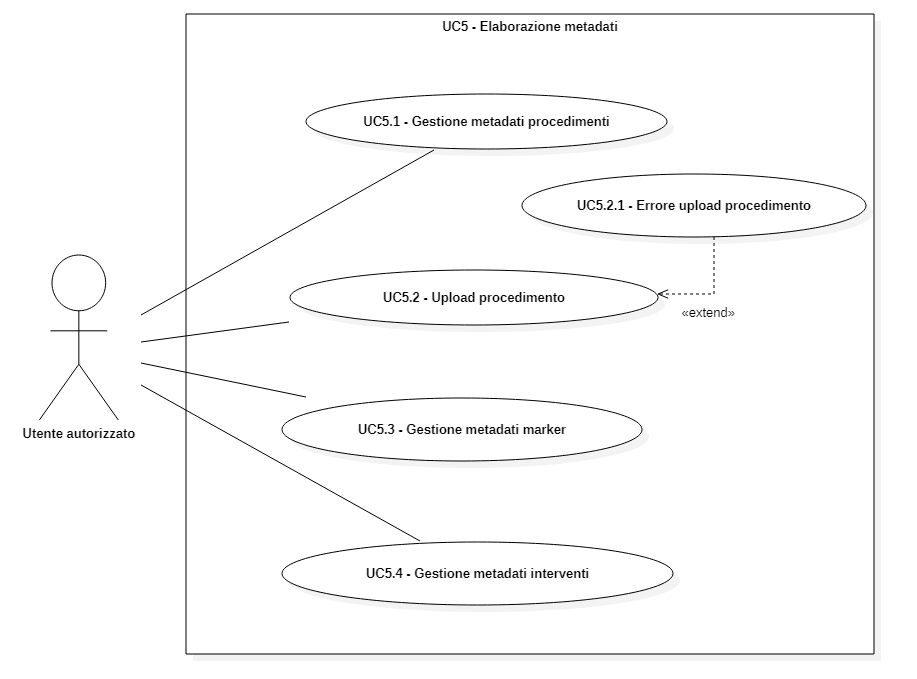
\includegraphics[scale=0.50]{images/UC5.png}
  \caption{Descrizione grafica caso d'uso UC5}
\end{figure}

\begin{itemize}
  \item \textbf{Attori}
        \begin{itemize}
          \item \textit{Primari}: utente autorizzato
        \end{itemize}
  \item \textbf{Precondizione}: l'utente si trova sulla pagina di visualizzazione dei dati.
  \item \textbf{Postcondizione}: l'utente ha caricato il procedimento desiderato e i relativi file.
  \item \textbf{Scenario principale}: l'utente tramite l'apposito bottone per l'upload, carica il procedimento desiderato.
  \item \textbf{Scenario secondario}: la procedura di upload procedimento non va a buon fine e restituisce un errore. (\textbf{UC5.1})
\end{itemize}

\subsubsection{UC5.1 - Errore upload procedimento}
\begin{itemize}
  \item \textbf{Identificativo}: UC5.1
  \item \textbf{Nome}: errore upload procedimento
  \item \textbf{Descrizione grafica}: (approfondita in UC5)
  \item \textbf{Attori}
        \begin{itemize}
          \item \textit{Primari}: utente autorizzato
        \end{itemize}
  \item \textbf{Precondizione}: il sistema non ha gestito correttamente la richiesta di upload procedimento.
  \item \textbf{Postcondizione}: l'errore viene visualizzato sull'applicazione.
  \item \textbf{Scenario principale}: la richiesta di upload procedimento non va a buon fine e l'errore viene mostrato all'utente.
\end{itemize}

% !TEX encoding = UTF-8
% !TEX TS-program = pdflatex
% !TEX root = ../tesi.tex
\begin{usecase}{6}{Visualizzazione Jobs}
  \usecaseactors{Utente autorizzato}
  \usecasepre{L'utente si trova all'interno dell'applicazione}
  \usecasedesc{Permette la visualizzazione dei jobs all'interno dell'applicazione}
  \usecasepost{L'utente può visualizzare i jobs}
  \label{uc:visualizzazione-jobs}
\end{usecase}
\begin{usecase}{7}{Visualizzazione singolo Job}
  \usecaseactors{Utente autorizzato}
  \usecasepre{L'utente si trova sulla pagina di visualizzazione dei jobs}
  \usecasedesc{Permette di visualizzare i dettagli del singolo job}
  \usecasepost{L'utente può visualizzare la pagina del singolo job}
  \label{uc:visualizzazione-job}
\end{usecase}


\subsection{UC6 - Visualizzazione jobs}
\begin{itemize}
  \item \textbf{Identificativo}: UC6
  \item \textbf{Nome}: visualizzazione jobs
  \item \textbf{Descrizione grafica}:
\end{itemize}

\begin{figure}[h]
  \centering
  %  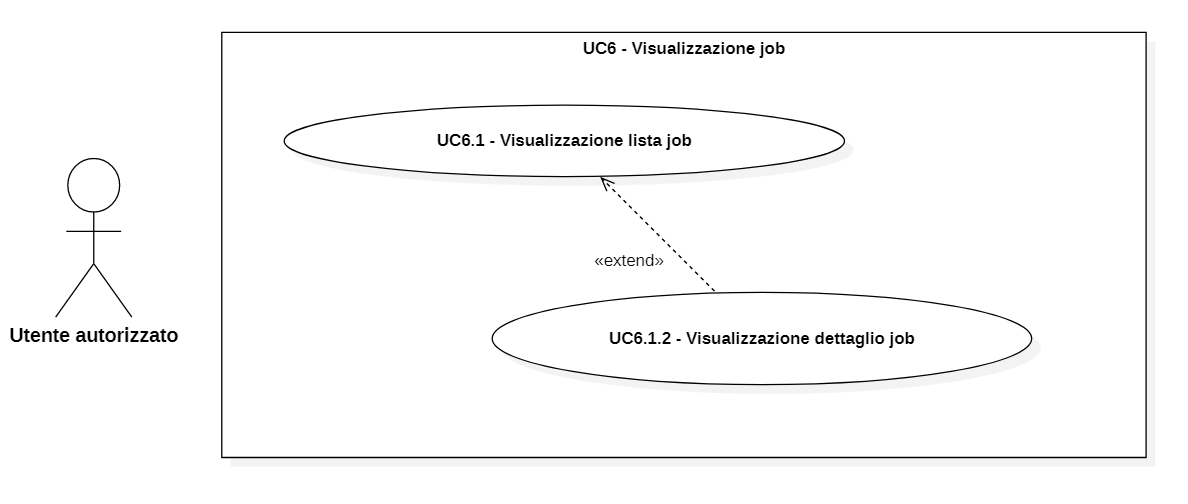
\includegraphics[scale=0.50]{images/UC6.png}
  \caption{Descrizione grafica caso d'uso UC6}
\end{figure}

\begin{itemize}
  \item \textbf{Attori}
        \begin{itemize}
          \item \textit{Primari}: utente autorizzato
        \end{itemize}
  \item \textbf{Precondizione}: l'utente si trova all'interno dell'applicazione e vuole visualizzare la lista dei jobs.
  \item \textbf{Postcondizione}: l'utente visualizza la lista dei jobs.
  \item \textbf{Scenario principale}: l'utente visualizza la lista dei jobs.
  \item \textbf{Scenario secondario}: l'utente può visualizzare il dettaglio di un singolo job premendo sull'apposito link. (\textbf{UC6.1})
\end{itemize}

\subsubsection{UC6.1 - Visualizzazione dettaglio job}
\begin{itemize}
  \item \textbf{Identificativo}: UC6.1
  \item \textbf{Nome}: visualizzazione dettaglio job
  \item \textbf{Descrizione grafica}: (approfondita in UC6)
  \item \textbf{Attori}
        \begin{itemize}
          \item \textit{Primari}: utente autorizzato
        \end{itemize}
  \item \textbf{Precondizione}: l'utente ha premuto sull'apposito link.
  \item \textbf{Postcondizione}: il dettaglio del job viene visualizzato.
  \item \textbf{Scenario principale}: l'utente visualizza tutti i dettagli del singolo job.
\end{itemize}


\section{Tracciamento dei requisiti}

Da un'attenta analisi dei requisiti e degli use case effettuata sul progetto è stata stilata la tabella che traccia i requisiti in rapporto agli use case.\\
Sono stati individuati diversi tipi di requisiti e si è quindi fatto utilizzo di un codice identificativo per distinguerli.\\
Il codice dei requisiti è così strutturato R(F/Q/V)(O/D/F) dove:
\begin{enumerate}
  \item[R =] requisito
  \item[F =] funzionale
  \item[Q =] qualitativo
  \item[V =] di vincolo
  \item[O =] obbligatorio
  \item[D =] desiderabile
  \item[F =] facoltativo
\end{enumerate}
Nelle tabelle \ref{tab:requisiti-funzionali} e \ref{tab:requisiti-qualitativi} sono riassunti i requisiti e il loro tracciamento con gli use case delineati in fase di analisi.
\newpage
\renewcommand{\arraystretch}{1.8} %aumento ampiezza righe
\begin{table}%
  \begin{tabularx}{\textwidth}{|l|X|c|}
    \hline
    \textbf{Requisito} & \textbf{Descrizione}                           & \textbf{Use Case} \\
    \hline
    RFO-1              & autenticazione                                 & UC1               \\
    \hline
    RFO-2              & lettura dati da CD                             & UC2               \\
    \hline
    RFO-3              & visualizzazione dati ordinati per file         & UC3               \\
    \hline
    RFO-4              & visualizzazione dati ordinati per procedimenti & UC4               \\
    \hline
    RFO-5              & gestione dei Marker relativi al file           & UC3               \\
    \hline
    RFO-6              & gestione degli Interventi relativi al file     & UC3               \\
    \hline
    RFD-1              & upload procedimento                            & UC5               \\
    \hline
    RFF-2              & visualizzazione jobs                           & UC6               \\
    \hline
    RFF-1              & riproduzione audio file                        & UC3.1             \\
    \hline
  \end{tabularx}
  \\
  \label{tab:requisiti-funzionali}
  \caption{Tabella del tracciamento dei requisti funzionali}
\end{table}%
\renewcommand{\arraystretch}{1.8} %aumento ampiezza righe
\begin{table}%
  \begin{tabularx}{\textwidth}{|l|X|l|}
    \hline
    \textbf{Requisito} & \textbf{Descrizione}    & \textbf{Use Case} \\
    \hline
    RQD-1              & test di unità esaustivi & -                 \\
    \hline
  \end{tabularx}
  \\
  \label{tab:requisiti-qualitativi}
  \caption{Tabella del tracciamento dei requisiti qualitativi}
\end{table}%